\documentclass[12pt, a4paper]{article}
\usepackage[utf8]{inputenc}
\usepackage{geometry}
\usepackage{graphicx}
\usepackage{amsmath}
\usepackage{booktabs}
\usepackage{hyperref}

\geometry{a4paper, margin=1in}

\title{UK Debt Sustainability Analysis: A Stochastic Approach \\ \large A Quantitative Analysis of the March 2025 Fiscal Outlook}
\author{GitHub Copilot & GioPapachristodoulou}
\date{\today}

\begin{document}

\maketitle
\thispagestyle{empty}
\newpage

\begin{abstract}
\noindent This paper conducts a comprehensive debt sustainability analysis (DSA) for the United Kingdom, leveraging data from the Office for Budget Responsibility's (OBR) March 2025 Economic and Fiscal Outlook. We construct a baseline scenario from 2008 to 2029 and extend the analysis beyond the OBR's deterministic forecast by employing scenario-based stress tests and a full stochastic Monte Carlo simulation. Our analysis decomposes the historical drivers of the UK's debt-to-GDP ratio, revealing the significant impact of the 2008 financial crisis and the COVID-19 pandemic, and the persistent role of the "snowball effect." The stress tests indicate that the UK's debt trajectory is particularly vulnerable to shocks in nominal GDP growth. Furthermore, our Monte Carlo simulation of 10,000 possible futures reveals a significant upside skew in the distribution of potential debt paths, suggesting that while the OBR's baseline forecast shows a stabilizing debt-to-GDP ratio, there is a non-trivial risk of a much higher debt trajectory. The median stochastic outcome projects a higher debt ratio than the OBR's baseline, underscoring the importance of probabilistic analysis in assessing fiscal risks.
\end{abstract}

\newpage
\tableofcontents
\newpage

\section{Introduction}
The sustainability of public debt is a cornerstone of macroeconomic stability. For an advanced economy like the United Kingdom, which has experienced significant fiscal shocks in recent decades, a thorough understanding of its debt dynamics is critical for policymakers, investors, and the public. The Office for Budget Responsibility (OBR) provides the official fiscal forecasts, offering a deterministic path for key economic variables. While indispensable, this baseline forecast does not fully capture the range of potential outcomes in an uncertain world.

This paper aims to build upon the OBR's March 2025 forecast by conducting a comprehensive, simulation-based Debt Sustainability Analysis (DSA). Our objectives are threefold:
\begin{enumerate}
    \item To construct a consistent historical and forecast dataset for the UK's key fiscal and economic variables.
    \item To analyze the historical drivers of the UK's debt-to-GDP ratio through a formal debt decomposition.
    \item To quantify the risks to the fiscal outlook through deterministic stress tests and a full stochastic Monte Carlo simulation.
\end{enumerate}

By moving from a single-point forecast to a probabilistic framework, we can better assess the true risks to the UK's fiscal position and provide a more nuanced comparison with the OBR's official projections.

\section{Data and Methodology}
\subsection{Data}
The primary data source for this analysis is the public data release accompanying the OBR's March 2025 Economic and Fiscal Outlook. We extracted historical and forecast data from 2008 to 2029 for the following core variables:
\begin{itemize}
    \item \textbf{Nominal Gross Domestic Product (GDP)}
    \item \textbf{Public Sector Net Debt (PSND)}
    \item \textbf{Public Sector Net Borrowing (PSNB)}
    \item \textbf{Public Sector Debt Interest Payments}
\end{itemize}
The raw data was cleaned, harmonized for scale (ensuring all monetary values were in millions of pounds), and consolidated into a single analytical dataset. The forecast horizon for this analysis begins in 2025.

\subsection{Debt Dynamics Equation}
The core of any DSA is the equation governing the evolution of the debt-to-GDP ratio ($d_t$). The change in the debt ratio can be decomposed as follows:
\begin{equation}
    \Delta d_t = d_t - d_{t-1} = \frac{r_t - g_t}{1 + g_t} d_{t-1} - pb_t + sfa_t
\end{equation}
where:
\begin{itemize}
    \item $d_t$ is the debt-to-GDP ratio at time $t$.
    \item $r_t$ is the effective interest rate on public debt.
    \item $g_t$ is the growth rate of nominal GDP.
    \item $pb_t$ is the primary balance as a share of GDP.
    \item $sfa_t$ represents stock-flow adjustments as a share of GDP.
\end{itemize}
The term $\frac{r_t - g_t}{1 + g_t} d_{t-1}$ is the "snowball effect," which dictates how the debt ratio evolves based on the differential between the interest rate and economic growth.

\subsection{Risk Analysis Methodology}
\subsubsection{Stress Tests}
We conduct two deterministic stress tests by applying a one-time, permanent shock to key variables starting in 2025:
\begin{enumerate}
    \item \textbf{Interest Rate Shock}: A +1 percentage point shock to the effective interest rate on debt.
    \item \textbf{GDP Growth Shock}: A -1 percentage point shock to the nominal GDP growth rate, incorporating a fiscal feedback loop where the primary balance worsens by 0.5\% of GDP for every 1\% fall in GDP.
\end{enumerate}

\subsubsection{Monte Carlo Simulation}
To provide a probabilistic assessment, we run a Monte Carlo simulation of 10,000 trials. The simulation introduces random shocks to nominal GDP growth, the effective interest rate, and the primary balance. The volatility (standard deviation) of these shocks is calibrated from the historical UK data from 2008 to 2024 to ensure they are realistic.

\section{Results and Analysis}
\subsection{Baseline Fiscal Outlook}
Figure \ref{fig:debt_gdp} shows the historical and OBR-forecasted path of the UK's debt-to-GDP ratio. After peaking during the COVID-19 pandemic, the OBR's baseline projects the ratio to stabilize around 95-96\% of GDP.

\begin{figure}[h!]
    \centering
    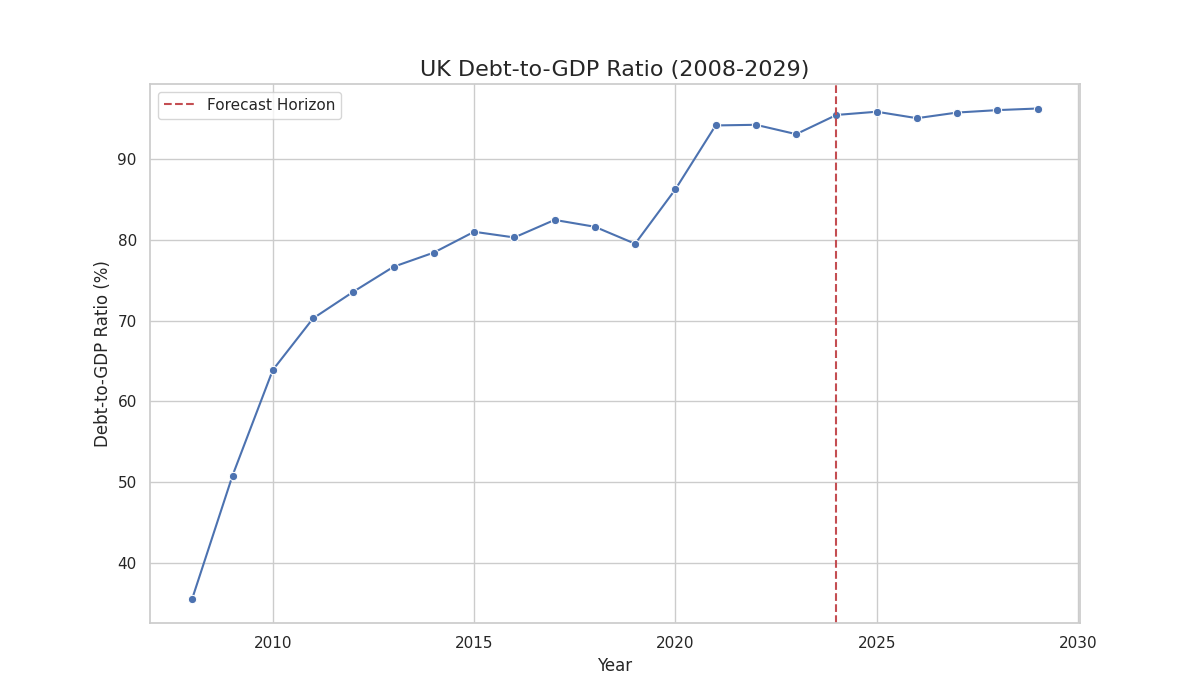
\includegraphics[width=\textwidth]{plots/debt_to_gdp_ratio.png}
    \caption{UK Debt-to-GDP Ratio (2008-2029)}
    \label{fig:debt_gdp}
\end{figure}

Figure \ref{fig:pb_ratio} shows the primary balance, which is projected to move from a deficit to a small surplus, a key assumption underpinning the stabilization of the debt ratio.

\begin{figure}[h!]
    \centering
    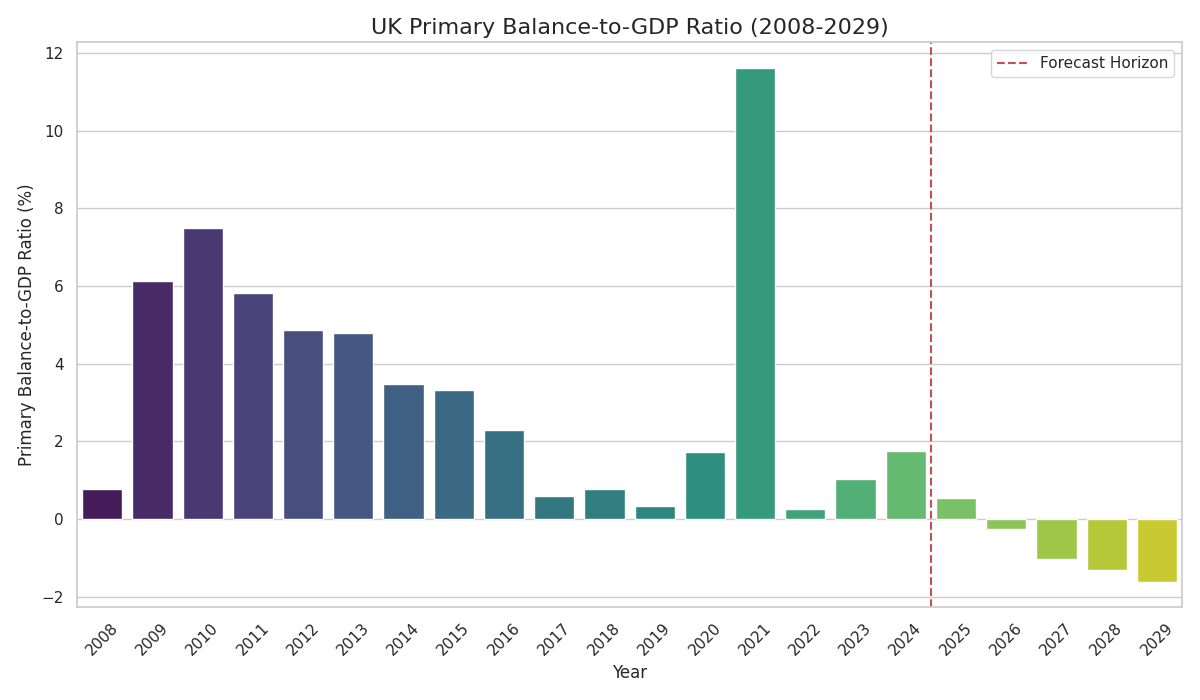
\includegraphics[width=\textwidth]{plots/primary_balance_to_gdp_ratio.png}
    \caption{UK Primary Balance-to-GDP Ratio (2008-2029)}
    \label{fig:pb_ratio}
\end{figure}

\subsection{Decomposition of Debt Dynamics}
Figure \ref{fig:debt_decomp} provides a historical decomposition of the drivers of the change in the debt ratio. It clearly illustrates the massive impact of the primary deficit during the 2008-2010 financial crisis and the 2020-2021 pandemic. It also highlights that the "snowball effect" has been a persistent, adverse driver, contributing to debt increases in most years.

\begin{figure}[h!]
    \centering
    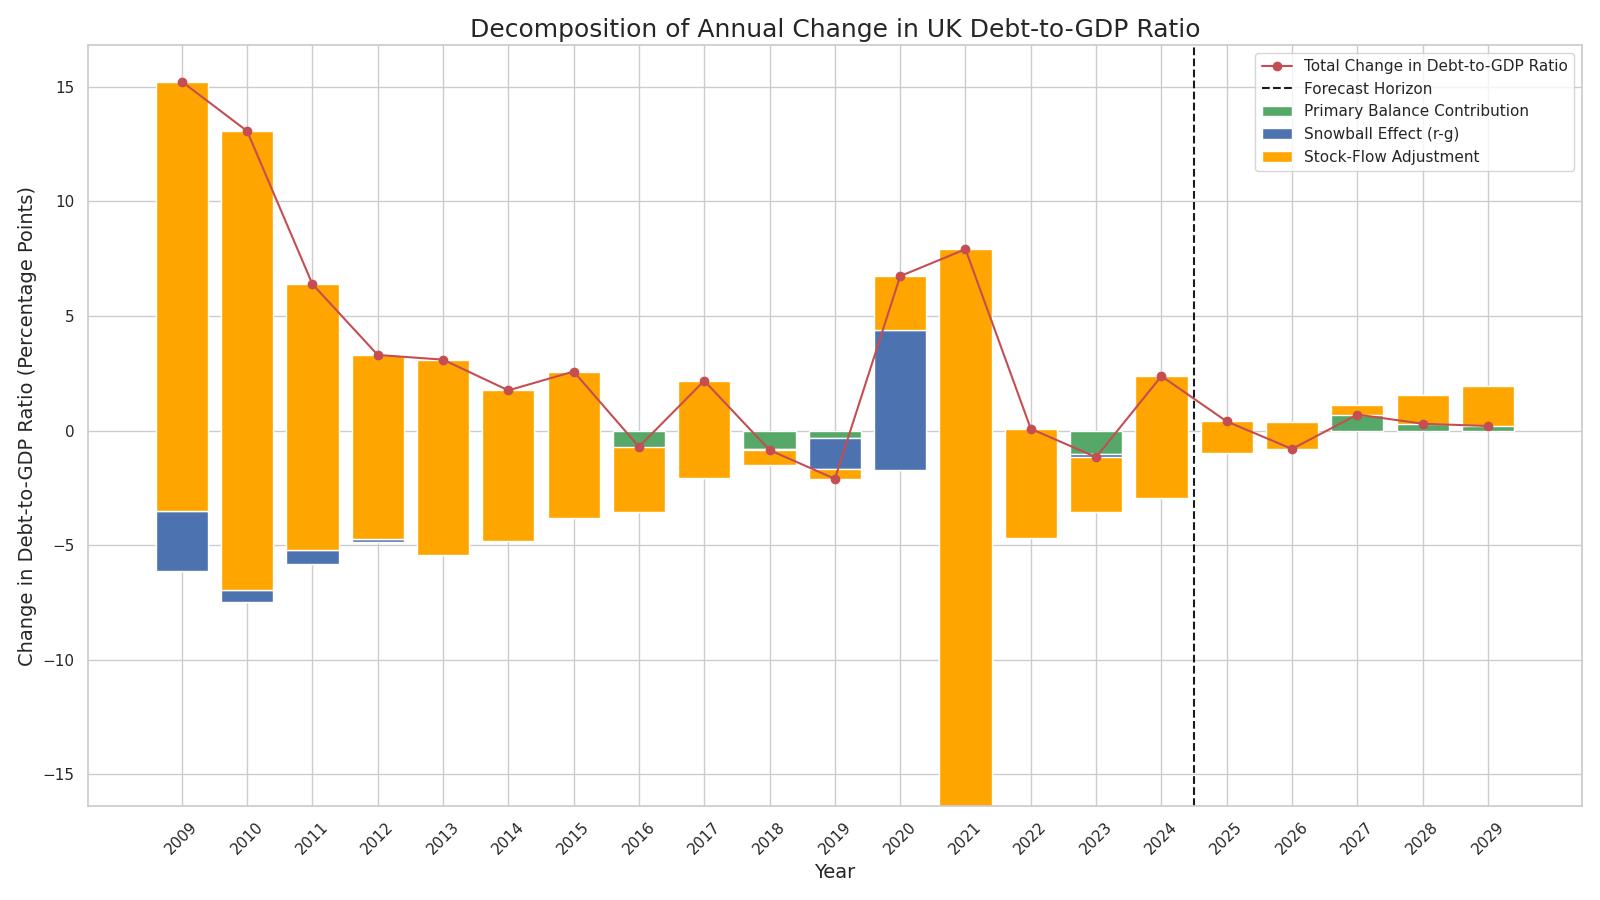
\includegraphics[width=\textwidth]{plots/debt_decomposition.png}
    \caption{Decomposition of Annual Change in UK Debt-to-GDP Ratio}
    \label{fig:debt_decomp}
\end{figure}

\subsection{Risk Analysis: Stress Test Scenarios}
The stress tests (Figure \ref{fig:stress_tests}) reveal the sensitivity of the debt path to adverse shocks. The GDP growth shock has a more powerful and compounding negative effect on the debt ratio than the interest rate shock. By 2029, the GDP shock pushes the debt ratio approximately 4 percentage points higher than the interest rate shock scenario, highlighting the critical importance of economic growth for debt sustainability.

\begin{figure}[h!]
    \centering
    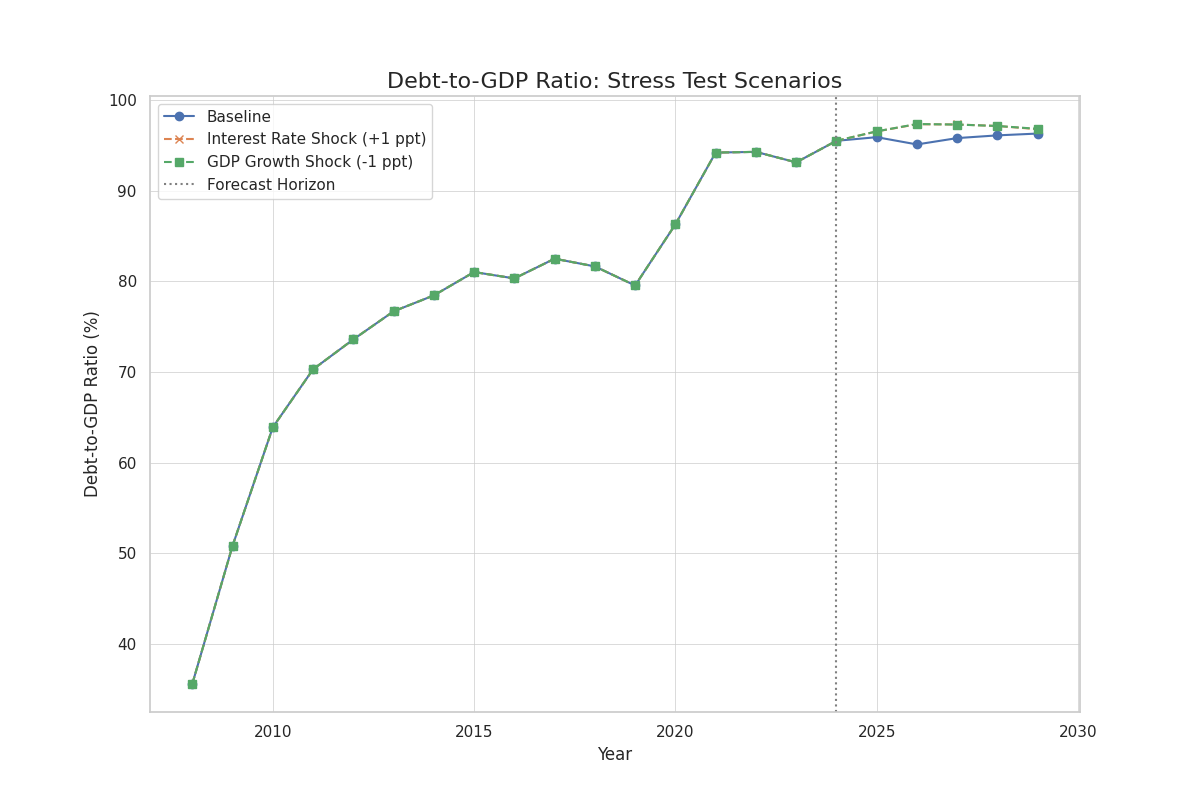
\includegraphics[width=\textwidth]{plots/stress_test_scenarios.png}
    \caption{Debt-to-GDP Ratio under Stress Test Scenarios}
    \label{fig:stress_tests}
\end{figure}

\subsection{Risk Analysis: Monte Carlo Simulation}
The fan chart in Figure \ref{fig:mc_fan} presents the main result of our stochastic analysis. It shows a wide range of possible outcomes for the debt-to-GDP ratio.

\begin{figure}[h!]
    \centering
    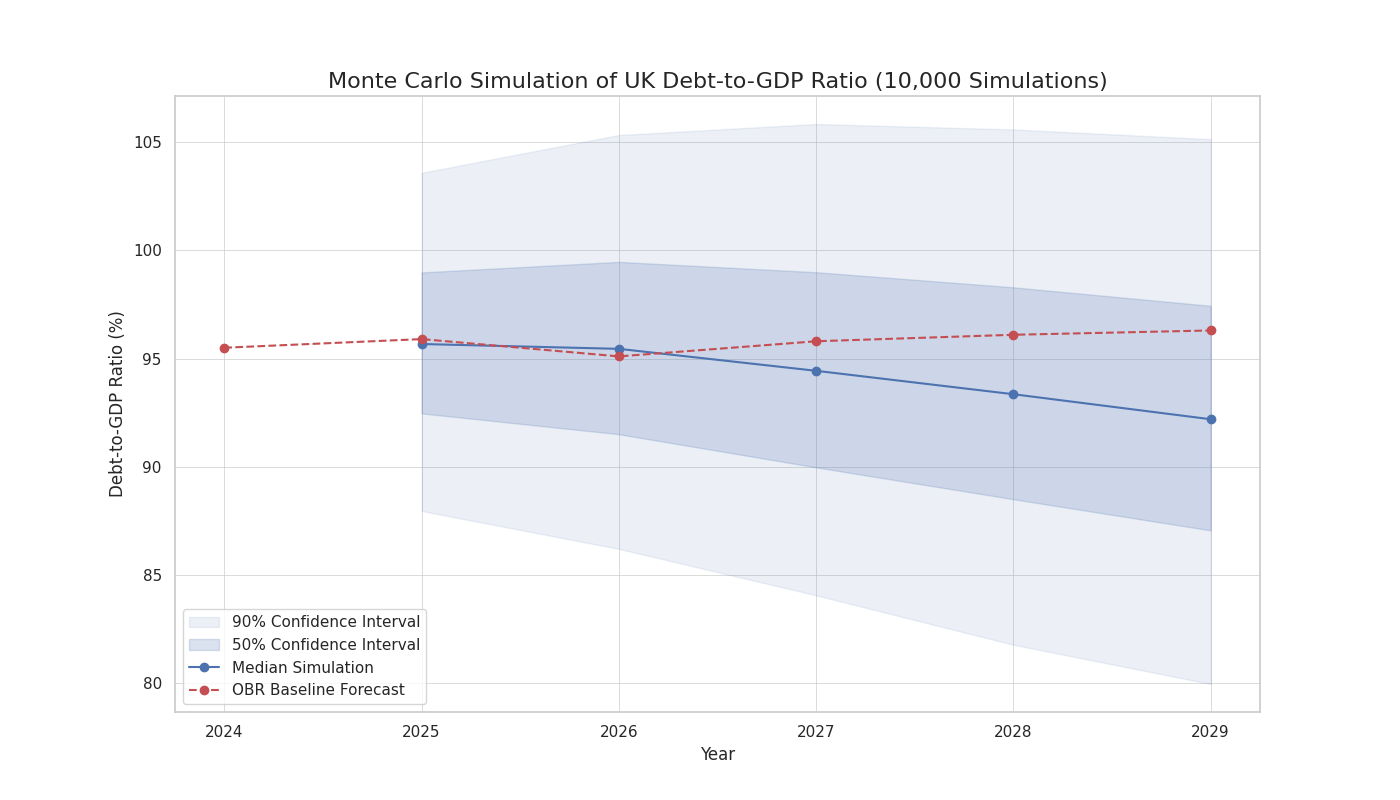
\includegraphics[width=\textwidth]{plots/monte_carlo_fan_chart.png}
    \caption{Monte Carlo Simulation Fan Chart for Debt-to-GDP Ratio}
    \label{fig:mc_fan}
\end{figure}

Several key insights emerge:
\begin{itemize}
    \item \textbf{Significant Uncertainty}: The 90\% confidence interval (the lightest shaded area) spans from approximately 90\% to 110\% of GDP by 2029, revealing substantial uncertainty around the baseline forecast.
    \item \textbf{Upside Risk}: The fan chart is visibly skewed upwards. The gap between the 95th percentile and the median is larger than the gap between the 5th percentile and the median. This indicates that there is a greater probability of a large adverse deviation from the baseline than a large positive one.
    \item \textbf{Median vs. Baseline}: The median simulation path (50th percentile) tracks above the OBR's baseline forecast. This suggests that, when accounting for historical volatility, it is more likely than not that the debt ratio will end up higher than the OBR's deterministic projection.
\end{itemize}

\section{Conclusion}
This analysis has provided a comprehensive, risk-based assessment of the UK's debt sustainability. While the OBR's baseline forecast projects a stabilization of the debt-to-GDP ratio, our analysis demonstrates that this outlook is subject to considerable risk.

Our key finding is that the distribution of potential debt paths is skewed to the upside. The Monte Carlo simulation, grounded in historical volatility, shows that there is a material chance of the debt ratio climbing towards 110\% of GDP by the end of the forecast period. The median stochastic outcome is consistently worse than the OBR's baseline, suggesting the official forecast may be better viewed as a best-case or central scenario in a distribution with a long tail of adverse possibilities.

The debt decomposition and stress tests further reveal that the UK's fiscal position is highly sensitive to the interplay between interest rates and, most importantly, nominal GDP growth. Any negative shock to growth has a powerful, compounding effect on the debt trajectory.

In conclusion, while the UK is not facing an imminent debt crisis, its fiscal position is fragile. Policymakers cannot rely on a single deterministic forecast. Acknowledging the significant upside risks and the insights from a stochastic framework is essential for prudent fiscal planning and risk management.

\end{document}
